%%%%%%%%%%%%%%%%%%%%%%%%%%%%%%%%%%%%%%%%%%%%%%
%Lab report writeup based on template by Derek Hildreth
%%%%%%%%%%%%%%%%%%%%%%%%%%%%%%%%%%%%%%%%%%%%%%

%\documentclass[aps,letterpape,10pt]{revtex4}
\documentclass[aps,letterpaper,10pt]{article}
%\documentclass{article}

\usepackage{graphicx} % For images
\usepackage{float}    % For tables and other floats
\usepackage{verbatim} % For comments and other
\usepackage{amsmath}  % For math
\usepackage{amssymb}  % For more math
\usepackage{fullpage} % Set margins and place page numbers at bottom center
\usepackage{subfig}   % For subfigures
\usepackage[usenames,dvipsnames]{color} % For colors and names
\usepackage{fancyhdr} %headers
\usepackage{listings} %for code
\usepackage{color} %to color code
\usepackage{wrapfig} % for inline images

%Color and code setup
\definecolor{dkgreen}{rgb}{0,0.6,0}
\definecolor{gray}{rgb}{0.5,0.5,0.5}
\definecolor{mauve}{rgb}{0.58,0,0.82}
\definecolor{codebg}{rgb}{.95,.95,.98}

\lstset{ %
	language=Python, 
	tabsize=4, 
	numbers=left,
	numberstyle=\footnotesize,
	backgroundcolor=\color{codebg},
	breaklines=true,
	breakatwhitespace=true,
	basicstyle=\small,
	numberstyle=\tiny\color{black},
	showstringspaces=false,
	keywordstyle=\color{blue}, 
	stringstyle=\color{dkgreen},
	commentstyle=\color{gray},
	frame=single,
	title = \texttt{\lstname}
	}

%%%%%%%%%%%%

%HEADER FORMATING%%%%%%%%%%%%%
\pagestyle{fancy}
\headheight 10pt
\setlength{\headsep}{20pt}
\lhead{MPHY 396 - Prof. Armato\\ Homework 2}
\rhead{A. Athanassiadis\\Due 1/25/2011}
%%%%%%%%%%%%%%%%%%%%%%%%

%Custom Definitions%%%%%%%%%%%%%%%
\newcommand{\ttt}{\texttt}
%%%%%%%%%%%%%%%%%%%%%%%%

\begin{document}
\section{Problem 1}
\begin{figure}[!h]
\centering
\subfloat[Original]{\label{fig:2-1a}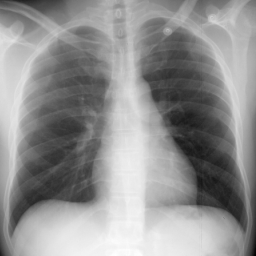
\includegraphics[width=128px]{2-1.png}}\hfill
\subfloat[Nearest-Neighbor Interpolation]{\label{fig:2-1b}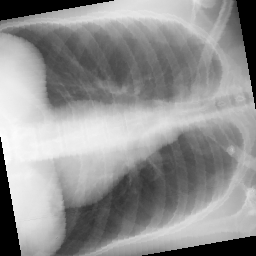
\includegraphics[width=128px]{2-1a.png}}\hfill
\subfloat[Linear Interpolation]{\label{fig:2-1c}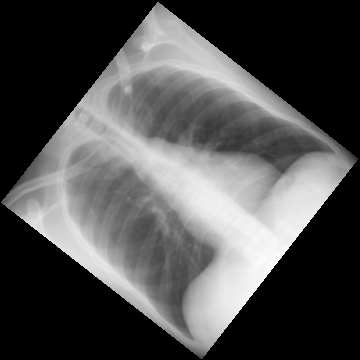
\includegraphics[width=128px]{2-1b.png}}
\caption{Image Rotation}
\label{2-1}
\end{figure}
In this problem, I created a \ttt{rotate()} function to rotate the original image by an arbitrary angle, $\theta$, given in degrees.  The rotate function takes an input image, and maps its points to those in a new image by rotating a point in the new image by $-\theta$ and then interpolating the result.  I allowed a few options, which included the interpolation scheme, and an image reshaping feature.  Figure \ref{fig:2-1b} demonstrates a rotation of $80^\circ$ about the center with nearest-neighbor interpolation.  Without the `reshape' flag set for this rotation, the edges were cropped to preserve the $256\times256$ original shape. Figure \ref{fig:2-1c} demonstrates a rotation of $-52^\circ$  with the reshaping feature, which calculates the size of the new image based on the rotation angle.  This image used linear interpolation, and resulted in a $360\times360$ image which was scaled above to fit on the page.

Comparing the two rotated images, the advantages of linear interpolation over nearest-neighbor are clear.  Nearest-neighbor interpolation introduces pixelation, especially noticeable on diagonal edges, whereas linear interpolation minimizes these effects.  Since the difference in computation time for these two is negligible,  linear interpolation seems to be the better algorithm to use.
\lstinputlisting{problem1.py}

\newpage
\section{Problem 2}
\begin{figure}[!h]
\centering
\subfloat[Original]{\label{fig:2-2a}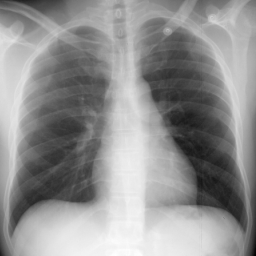
\includegraphics[width=200px]{2-2.png}} \hspace{20px}
\subfloat[Edge Magnitude]{\label{fig:2-2b}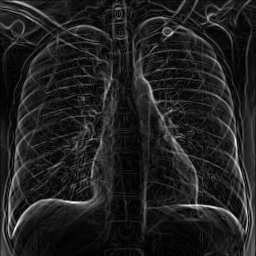
\includegraphics[width=200px]{2-2a.png}}  \\
\subfloat[8-bit Edge Direction]{\label{fig:2-2d}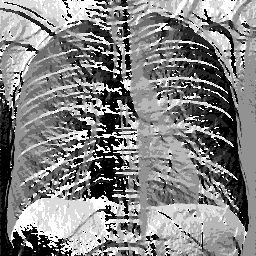
\includegraphics[width=200px]{2-2b.png}} \hspace{20px}
\subfloat[Edge Magnitude Contrast]{\label{fig:2-2c}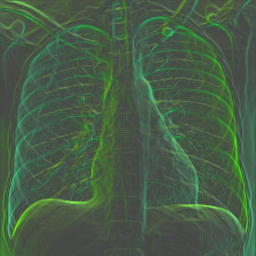
\includegraphics[width=200px]{2-2c.png}} 
\caption{Edge Calculations}
\label{2-2}
\end{figure}
Here, I used the Sobel filters, $h_1,\ h_2,\ h_3$ (Sonka, p.146) to perform edge detection on the original image.  If $x$ denotes the image response to $h_1$ and $y$ the response to $h_3$, then the magnitude image (Figure \ref{fig:2-2b}) was calculated using $I_M=\sqrt{x^2+y^2}$.  Figure \ref{fig:2-2c} shows another rendering of the magnitude image, where the blue shades indicate where the $h_1$ response was strongest and the yellow shades represent where the $h_3$ response was strongest.  Stronger green represents where both filters had equal response. The direction image (Figure \ref{fig:2-2d}) was calculated using $I_D=\text{\ttt{arctan2}}(\frac{x}{y})$, where  \ttt{arctan2()} is an implementation of the \ttt{arctan()} function that preserves quadrant information.  The output from \ttt{arctan2()} was further processed, binning it by angle.  The result is an octary image where each grayscale level represents a direction as seen in Figure \ref{fig:encodings}.
\begin{figure}[!h]
\centering
\begin{minipage}[c]{3cm}
\centering
\renewcommand{\arraystretch}{1.5}
\renewcommand{\tabcolsep}{0.2cm}
\begin{tabular}{|c|c|c|}
\hline
3 & 2 & 1 \\
\hline
4 & $\times$ & 0 \\
\hline
5 & 6 & 7\\
\hline
\end{tabular}
\end{minipage}
\begin{minipage}[c]{3cm}
\centering

\includegraphics[width=2cm]{imguide.png}
\end{minipage}
\caption{Direction Encoding}
\label{fig:encodings}
\end{figure}

It is important to note that there is a loss of information when encoding in this way. At a point where the edge magnitude is zero, the direction image still contains a value between 0 and 8.  Because there is no way to encode a pixel in the middle of a constant grey-value region, this information is lost in the encoding, and can only be determined if edge magnitude image is provided with the direction image.
Also, the noise in edge direction is apparent in Figure \ref{fig:2-2c}.  This noise can be reduce by blurring the input image with a smoothing kernel, and then performing edge detection.  However, blurring generally lowers the edge magnitude.

\lstinputlisting{problem2.py}

\section{Appendix: Common Code}
Common functions used for these problems are contained in \texttt{preprocessing.py}.
\lstinputlisting{preprocessing.py}

\end{document} 